\section{Introduction}
\label{intro}
Natural language is rife with ambiguities. A word or a phrase usually has
multiple meanings depending on the context of its use.
This has been one of the most
significant problems in automatic understanding and processing of human
text.
%One of the key steps in automatically understanding
%human text to disambiguate phrases, or says multi-word expressions(MWE)
%in sentences. Since MWEs are important semantic components for
%understanding a whole sentence.
Consider the following sentences.
\myskip
\begin{example}
\label{ex-bear1}
%{\em
%Watch the largest land carnivore, \textbf{polar bear} and
%its cubs, hunting for food and swimming in the sea.
The \textbf{polar bear} is a bear native largely within the \uline{Arctic Circle}
encompassing the \uline{Arctic Ocean}, its surrounding seas and surrounding \uline{land masses}.
%}
\end{example}
\begin{example}
\label{ex-bear2}
%{\em
The original band, \textbf{Polar Bear}, was formed in 1994 by
\uline{Gary Lightbody} who was a student at \uline{Dundee University} in Scotland.
%}
\end{example}
%\myskip

In \exref{ex-bear1}, ``polar bear'' refers to a large white carnivorous
bear inhabiting the arctic region; in \exref{ex-bear2}, ``Polar Bear'' is
the former name of a British rock band. The task of labeling
a word or a {\em multi-word expressions} (MWE) (collectively called
as a {\em term}) in a plain text by their explicit meanings
is known as {\em phrase sense disambiguation}
(PSD) problem \cite{carpuat2007phrase}.
%known as {\em sense labeling}, which explicitly
%labels the meaning of a phrase given its surrounding context.
PSD generalizes the more well-known open problem,
{\em word sense disambiguation} (WSD)~\cite{navigli09:wsd}, which seeks
to identify the meaning or the {\em sense} of the {\em words}.
The difference is that in WSD, the disambiguated unit is word, not phrase.

PSD is an important generalization because
the meanings of MWEs can be independent of the constituent words so traditional
WSD techniques cannot be directly applied on PSD problems. For example,
the word ``masses''  often means normal people, while the term ``Dundee''
usually reminds us of the hilarious Australian comedy from the 80's, and
neither of these meanings have anything to do with ``land masses''
or ``Dundee University'' above.
%Also, a research done by Carpuat, M.\cite{carpuat2007phrase} shows that
%PSD help statistical machine
%translation better than WSD.
In fact, some researchers have already indicated that
PSD outperforms WSD in NLP tasks such as statistical
machine translation \cite{carpuat2007phrase}.
Moreover, the number of MWEs is massive. For example, if we consider
Wikipedia \cite{wikipedia},
which is the largest online encyclopedia there is today with
over 4 million concepts (articles), 62.8\% of the concept terms (titles
of the articles) consist of two or more words. %(See \figref{fig:numwords}).
A random sample of 10,000 web pages suggests that 66.2\%
of the phrases in them are ambiguous, because they can be mapped to
two or more concepts in Wikipedia.

%\begin{figure}[th]
%\centering
%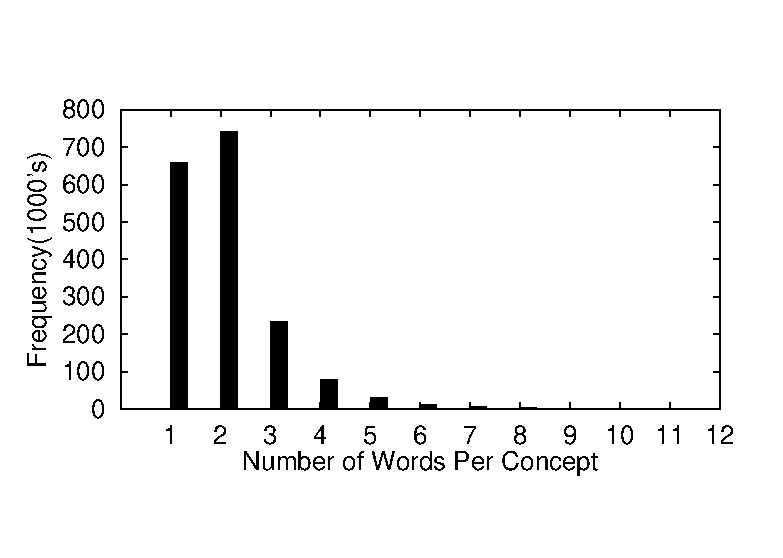
\epsfig{file=figure/histogram.eps,width=0.7\columnwidth}
%\caption{Distribution of Concept Term Length in Wikipedia}
%\label{fig:numwords}
%\end{figure}

A particularly important form of PSD is known as
{\em wikification} \cite{MihalceaC07}. Wikification is an automatic process
of linking {\em every} possible MWE
in a document to an article in Wikipedia. This process
disambiguates the terms because the process is equivalent to labeling
a term with a proper sense (or concept) \footnote{In this paper,
we use the terms ``term'', ``MWE'' and ``phrase'' interchangeably.
We also use the terms ``sense'' and ``concept'' interchangeably.}
which is represented by a Wikipedia article.
Note that while almost all Wikipedia
concepts are noun-based, a small number of verbs or verb phrases are redirected to
their corresponding noun-phrase concepts (e.g., ``minimize'' is redirected to
the article ``Maxima and minima'').
Existing wikification techniques focus on noun-phrases because Wikipedia
does not have articles to support all senses of verbs or verb phrases.
For this reason, in the rest of the paper, when we mention ``terms'' or
MWEs, we mean noun phrases.

%In other words, concepts (articles) in Wikipedia are the possible senses
%for any given term.
%Given an input plain text document, we convert it into something similar
%to a Wikipedia page with as many proper links as possible.

%Our approach attacks the first drawback of word co-occurrence
%because wikification can be
%thought of as a generalization of WSD to
%include multi-word expressions or phrases
%into the disambiguation process as well. We call this general problem
%{\em Phrase Sense Disambiguation} or PSD.
%In this paper, we restrict
%ourselves to {\rm noun phrase} disambiguation, because most concepts in
%Wikipedia are noun phrases and they make up the majority concepts of any
%human language. It is possible, however, to combine wikification
%with another data source like WordNet to disambiguate other
%types of terms.

%The approach attacks the second drawback because
%Wikipedia \cite{wikipedia} is by far the largest dictionary and
%thesaurus for nouns and noun phrases, with over 4 million unique concepts and
%their definitions as of mid-2012. Each Wikipedia article describes a
%concept. Within an article, many terms are linked to other Wikipedia
%articles. Each such link provides the natural labeling for the surface
%forms of the term (i.e., the anchor text) and the sense is the linked articles.
%Instead of computing and storing word co-occurrence as knowledge,
%we can compute the {\em co-occurrences
%between senses} by looking at the links in the Wikipedia articles directly.
%This co-occurrence information is more reliable and easier to compute.
%In addition, Wikipedia provides disambiguation pages which lists all
%the known senses of a given term. We can use this information along with the
%sense co-occurrence for disambiguation.
%}

Previous work on wikification often models a Wikipedia concept by a {\em bag of
words} from its article, models a target term by its context
which is also a bag of words, and then compare the two bags.
The bag-of-words model doesn't work well
(e.g. on Example \ref{ex-bear1} and \ref{ex-bear2}) because:
1) many words themselves are ambiguous and many words don't offer distinctive
signals which means the combined signals from a bag are often convoluted.
(e.g., ``circle'',``bear'' and ``masses'' in \exref{ex-bear1}
all have multiple senses, and the words ``surrounding'',
``original'' and ``formed'' don't contribute much to the meaning of the
sentences).
2) it ignores other MWEs in the context or article by only treating them
as individual words which can misunderstand
some of the MWEs (e.g. ``land masses'' in \exref{ex-bear1}
and ``Dundee University'' in \exref{ex-bear2}).

An improvement over the above bag-of-words approach
uses the relatedness between two concepts to constraint
the labeling of two neighboring terms simultaneously
\cite{Tonelli2012,RatinovRDA11,kulkarni2009collective}. %\KZ{cite here}
The relatedness can be computed from the article inter-link graph structure
induced from the corpus\cite{ferragina2010tagme}.%\KZ{cite here also}
While the link structure is an important data source to extract
relation among concepts, the above approach misses out a more
{\em direct} and {\em accurate} source of information,
which is the {\em co-occurrence} between Wikipedia concepts in the corpus.
Such co-occurrence can be computed
by the co-occurrence of links within an article, a paragraph, or a predefined window,
since the links are the natural labels of surface terms to the concepts.

In this paper, we will show that wikification using link co-occurrence has
major advantages over all previous attempts.
We propose a novel and simple approach to the wikification problem
by using co-occurrence between Wikipedia links, and show that it is
much more effective and practical than all existing approaches.


%Computing link co-occurrences and the link structure both
%rely heavily on the correctness of link distribution in the corpus.
%For example, given two neighboring terms $t_1$ and $t_2$ where $t_1$ has
%two concepts $c_{11}$ and $c_{12}$ while $t_2$ has one concept $c_2$,
%if $re(c_{11}, c_2) \ge re(c_{12}, c_2)$, then $t_1$ is more likely to mean
%$c_{11}$ in the present context. So far, existing work calculates
%$re(c_1, c_2)$ often by the structure of the Wikipedia link network or
%category tree, e.g., some form of distance between the two concept nodes
%on the link graph.

Unfortunately, Wikipedia articles can be {\em sparsely linked}.
Some surface terms don't have a corresponding Wikipedia page
to link because it's not created yet; many others are not linked because either
they are too common or they have been linked previously in the article before.
Either way, the author of the article didn't consider them to be
``link-worthy''. Sparsely linked Wikipedia does not reveal the true
link distribution or link graph structure, and seriously harms
the accuracy of the link co-occurrence information.
Previous research on WSD using word
co-occurrence \cite{Stokoe2003:WSD} already indicated that
the correct distribution of a term's surrounding environment in
critical to the end-to-end disambiguation accuracy.
The same argument applies to wikification by concept co-occurrence.
%It is perhaps because of this, none of the previous wikification techniques
%attempted to use link co-occurrences to model relatedness.

%
%When we compute word co-occurrence in a text corpus, we can obtain an
%accurate context distribution because every word is counted
%in the context or ``window.'' Link co-occurrence information computed from these
%sparsely linked articles can be inaccurate
%and this risks the accuracy of the end-to-end wikification result.

To mitigate this problem, in this paper, we propose an iterative enrichment
algorithm that adds the {\em missing links} to Wikipedia pages. In a nutshell, this
algorithm maintains a concept co-occurrence matrix of the Wikipedia
snapshot in the current iteration as partial information, and
use it to disambiguate unlinked terms for the next iteration until
no more links can be added.
\figref{fig:beforeafter} shows a snapshot of the links in a sentence of a
Wikipedia article ``before'' and ``after'' the iteration process.
%In the bottom of the figure, we show the links our system added
%after the iterative process from surface form to senses with arrows.
%The sentence comes from the article of ``modern portfolio theory''.
%Before the enrichment, the sentence is very sparse with links while
%after the process, 10 links are added with high accuracy.
%Furthermore, a Wikipedia corpus with added links not only provides better
%link distribution but also induces a more accurate link network structure,
%which can improve the results of previously discussed approaches that rely
%on link structures or link distributions.
We have experimentally verified (in \secref{sec:eval}) that
our iterative enrichment algorithm increases the number of links by five times,
and the number of co-occurrence by three times,
and the final co-occurrence information thus produced
gives rise to significant improvement (up 17\% increase)
in the accuracy of end-to-end wikification.

\begin{figure}
\centering
\fbox{
\begin{minipage}{0.9\columnwidth}
{\scriptsize \tt
\textsf{
Modern portfolio theory(MPT) is a theory of {\color{blue}\uline{investment}} which attempts to maximize portfolio expected {\color{blue}\uline{rate of return}} for a given amount of portfolio risk, or equivalently minimize {\color{blue}\uline{financial risk}} for a given level of expected return, by carefully choosing the proportions of various {\color{blue}\uline{asset}}s.}
}
\end{minipage}
}
\vspace*{2ex}

%\fbox{
%\begin{minipage}{0.9\columnwidth}
%{\scriptsize \tt
%\textsf{
%{\color{blue}\uline{Modern portfolio theory}}[Modern portfolio theory] ({\color{blue}\uline{MPT}}[Modern portfolio theory]) is a {\color{blue}\uline{theory}}[Theory] of {\color{blue}\uline{investment}} which attempts to maximize {\color{blue}\uline{portfolio}}[Portfolio] expected {\color{blue}\uline{rate of return}} for a given {\color{blue}\uline{amount}}[Quantity] of {\color{blue}\uline{portfolio}}[Portfolio] {\color{blue}\uline{risk}}[Risk], or equivalently minimize {\color{blue}\uline{financial risk}} for a given {\color{blue}\uline{level}}[Level] of {\color{blue}\uline{expected return}}[Expected return], by carefully choosing the {\color{blue}\uline{proportions}}[Proportionality] of various {\color{blue}\uline{asset}}s.}
%}
%\end{minipage}
%}
\fbox{
\begin{minipage}{0.9\columnwidth}
{\scriptsize \tt
\textsf{
{\color{blue}\uline{Modern portfolio theory}}({\color{blue}\uline{MPT}}) is a {\color{blue}\uline{theory}} of {\color{blue}\uline{investment}} which attempts to maximize {\color{blue}\uline{portfolio}} expected {\color{blue}\uline{rate of return}} for a given {\color{blue}\uline{amount}} of {\color{blue}\uline{portfolio}} {\color{blue}\uline{risk}}, or equivalently minimize {\color{blue}\uline{financial risk}} for a given {\color{blue}\uline{level}} of {\color{blue}\uline{expected return}}, by carefully choosing the {\color{blue}\uline{proportions}} of various {\color{blue}\uline{asset}}s.}
}
\end{minipage}
}
\scriptsize

%\begin{flushleft}
%\begin{tabular}{lll}
%\myurl{Modern portfolio theory} & $\rightarrow$ &\textsf{[Modern portfolio theory]} \\
%\myurl{MPT} & $\rightarrow$ & \textsf{[Modern portfolio theory]}
%\end{tabular}
%\end{flushleft}
%\begin{tabular}{llllll}
%\myurl{theory} & $\rightarrow$ & \textsf{[Theory]} &
%\myurl{portfolio} & $\rightarrow$ & \textsf{[Portfolio]} \\
%\myurl{amount} & $\rightarrow$ & \textsf{[Quantity]} &
%\myurl{risk} & $\rightarrow$ & \textsf{[Risk]} \\
%\myurl{level} & $\rightarrow$ & \textsf{[Level]}  &
%\myurl{expected return} & $\rightarrow$ & \textsf{[Expected return]} \\
%\myurl{proportion} & $\rightarrow$ & \textsf{[Proportionality]}
%& & \\
%\end{tabular}

\vspace{0.2cm}
\begin{tabular}{llllllllll}
\multicolumn{4}{l}{\myurl{Modern portfolio theory}} & $\rightarrow$ & \multicolumn{4}{l}{\textsf{[Modern portfolio theory]}} &\\
\multicolumn{4}{l}{\myurl{MPT}} & $\rightarrow$ & \multicolumn{4}{l}{\textsf{[Modern portfolio theory]}} &\\
\multicolumn{2}{l}{\myurl{theory}} & $\rightarrow$ & \multicolumn{2}{l}{\textsf{[Theory]}} &
\multicolumn{2}{l}{\myurl{portfolio}} & $\rightarrow$ & \multicolumn{2}{l}{\textsf{[Portfolio]}} \\
\multicolumn{2}{l}{\myurl{amount}} & $\rightarrow$ & \multicolumn{2}{l}{\textsf{[Quantity]}} &
\multicolumn{2}{l}{\myurl{risk}} & $\rightarrow$ & \multicolumn{2}{l}{\textsf{[Risk]}} \\
\multicolumn{2}{l}{\myurl{level}} & $\rightarrow$ & \multicolumn{2}{l}{\textsf{[Level]}}  &
\multicolumn{2}{l}{\myurl{expected return}} & $\rightarrow$ & \multicolumn{2}{l}{\textsf{[Expected return]}} \\
\multicolumn{2}{l}{\myurl{proportion}} & $\rightarrow$ & \multicolumn{2}{l}{\textsf{[Proportionality]}} & & & & &
\end{tabular}

\caption{Snapshot of a Wikipedia article ``before'' and ``after'' iteration.
The source and destination of newly added links
are indicated at the bottom.}
\label{fig:beforeafter}
\end{figure}
%\KZ{Maybe we can add two pics
%of ``before'' and ``after'' for a real wiki page.}



There are two other technical challenges in our wikification framework.
First, parsing of plain text into phrases can be ambiguous itself and
common NLP tools are not accurate enough in this chunking process.
%\KZ{Maybe give an example here?}
Considering the sentence in \exref{ex-rim}:
\begin{example}
\label{ex-rim}
{\em \textit{Snow Patrol are an alternative rock band formed
at the University of Dundee in 1994, though at this time as an indie
rock band, the band is now based in Glasgow, Scotland.}}
\end{example}
The phrase ``University'' and ``Dundee'' are treated as independent chunks in
the NLP chunker while ``University of Dundee'' is a correct parse.
\cut{
Second, the links to concepts in Wikipedia are not evenly distributed:
some popular and ``difficult'' concepts get linked way more often than others,
especially those common and ``easier'' terms.
E.g. ``country'' is a very common word, but the article ``Country'',
which is represents a region is rarely linked,
whereas the other sense ``Country music'', is linked 60 times more.
Such statistics causes algorithm to prefer difficult or rare concepts
than simple and more general ones
which harms the precision in wikification.
}

Second, wikifying a new, unlinked document is
a computationally intensive task because there's no support for
any sense so all combinations of senses must be attempted.
Suppose we have $n$ phrases in a sentence, each has $k$ senses in average,
the number of combination is $k^n$!
Thus, we need a method that balances accuracy with complexity.
%\KZ{Is there any other challenges, the above sounds not challenging enough!}

%Word Sense Disambiguation(WSD)\cite{navigli09:wsd} whose task is to identify the meaning
%of words in a given context. The motivation of WSD is that human language is ambiguous, one
%word in different context may have different meanings. For example, considering the following
%two sentences:
%\begin{itemize}
%\item Apple and Microsoft are two IT companies.
%\item Apple is a kind of delicious fruit.
%\end{itemize}
%[need more explanation when a good example is found]

This paper makes the following contributions.
\begin{enumerate}
\item We propose an iterative algorithm that disambiguates
unlinked MWEs in existing Wikipedia articles
by linking them to other appropriate
Wikipedia articles (concepts), and effectively enriches the link
distribution;
\item We propose a sliding-window based method to wikify a given
plain text document using the co-occurrence information obtained from
enriched Wikipedia corpus;
\item We show comprehensive evaluation results that demonstrate the
effectiveness of this novel approach with a web demo
\footnote{Wikification demo website:
\url{http://202.120.38.145:4082/wvc/Guess.aspx}.},
as shown in \figref{fig:screen-bear}.
\end{enumerate}

%\figref{fig:screen-bear} shows an example of wikifying the second
%example sentence above. Noun phrases that are identified are
%highlighted in yellow background and its meaning in Wikipedia is
%enclosed in the square brackets.
%Note that ``Polar Bear'' has been successfully
%labeled as {\em Snow Patrol}, the rock band.
\begin{figure}
\centering
\epsfig{file=screen-bear.eps,width=\columnwidth}
\caption{Result of Wikifying Example \ref{ex-bear2} via Link Co-occurrence.
Concepts are enclosed in square brackets.}
\label{fig:screen-bear}
\end{figure}

%\subsection{Paper Organization}
The rest of the paper is structured as follows.
\secref{sec:framework} presents
the algorithms of this framework;
\secref{sec:implement} discusses some implementation
details and optimizations;
\secref{sec:eval} demonstrates the experimental results;
\secref{sec:related} introduces some related work while
\secref{sec:conclude} concludes the paper.


%[Outline]
%
%\KZ{I revised the outline. Please follow this:}
%
%\begin{enumerate}
%\item What is wikification and why it's important (here you
%relation with WSD, the reliability of wikipedia sources, etc.)
%
%\item What are the existing techniques in wikification and also WSD
%and what are the deficiencies of these techniques.
%
%\item What are the challenges in Wikification/WSD?
%
%\item Briefly describe the key ideas in our approach (the punch line):
%(1) Building reliable coocurrence matrix of wiki concepts
%(2) Use sliding window algo to ``guess'' the meaning of terms in new text.
%
%\item Main contributions: (1) An iterative algo to add links to wiki corpus
%(2) a way solve the common terms problem (3) a sliding window algo to control
%the computation space while achieving local optimal solution in WSD.
%\end{enumerate}

%{\bf Our main arguments}
%
%\begin{enumerate}
%\item Co-occurrence is important (knowledge) for disambiguation
%\item word-based co-occurrence has two problems:
%	(1) requires massive labeling (supervised) or a large thesaurus
%	(wordnet)
%	(2) words can't capture some meanings expressed by phrases
%\item Co-occurrence of concepts (multiple-word phrase) is better than
%co-occurrence of words
%\item Co-occurrence obtained from the current wikipedia pages is
%insufficient
%\item Co-occurrence of concepts is a difficult problem: (1) ambiguity
%(2) general forms
%\item A window-based wikification algo can quickly tag/disamiguate a document.
%\end{enumerate}
%Nowadays internet outputs huge amount of textual documents in natural languages
%everyday, which contain a great deal of information and human knowledge. To
%effectively unlock this precious information,
%we need to enable machines to process
%and understand human text.

%Much work has been done on WSD. Since to identify the sense of a word
%essentially boils down to {\em understanding} its context, most approaches
%to WSD require some form of knowledge. One common form of knowledge
%is the co-occurrence information
%\cite{GuthrieGWA91,Li1998:wcd,ChungKML01,
%Stokoe2003:WSD,Fernandez-AmorosGSS10}
%extracted from text corpuses, e.g.,
%dictionary definitions \cite{LDOCE,Oxford}, news collections
%\cite{Charniak00:wsj} or even the web texts \cite{Brants06:web1t}.

%A great deal of information and human knowledge is stored in massive
%amount of textual documents in natural languages, many of which are in
%electronic forms. To effectively unlock this precious information, we
%must enable machines to process and understand human text.
%
%One of the key steps in understanding text is {\em word sense
%  disambiguation} (WSD)~\cite{navigli09:wsd}, which tries to identify
%the meaning or the {\em sense} of the words, given that many of them
%has more than one meanings (senses). According to the words' surrounding
%context, we explicitly label the meaning of them.
%
%%Consider the following sentences.
%%\myskip
%%\begin{example} \label{ex:bear-accept}
%%{\em The criminals must \textbf{bear} full responsibility for the innocent
%%deaths.}
%%\end{example}
%%\begin{example}
%%{\em US-based ETFs might lift you from the \textbf{bear} to the bull.}
%%\end{example}
%%\myskip
%%
%%Here, depending on the context,
%%%``bear can be large animal or a financial market trend.
%%``bear'' can be a verb which means {\em accept}, or a noun that means
%%{\em a financial market trend}. In this paper, we are concerned with a
%%common task in WSD known as {\em sense labeling}, which explicitly
%%labels the meaning of a word given its surrounding context.
%%Unless otherwise noted, WSD or disambiguation refers to sense labeling
%%in the rest of this paper.
%
%\subsection{Co-occurrence for WSD}
%Much work has been done on WSD.
%Despite years of effort, WSD remains an open problem.
%Because to identify the sense of a word essentially boils down to
%{\em understanding} its context, most approaches to
%WSD require some form of knowledge. One common form of knowledge
%is the co-occurrence information
%\cite{GuthrieGWA91,Li1998:wcd,ChungKML01,
%Stokoe2003:WSD,Fernandez-AmorosGSS10}
%extracted from text corpuses, e.g.,
%dictionary definitions \cite{LDOCE,Oxford}, news collections
%\cite{Charniak00:wsj} or even the web texts \cite{Brants06:web1t}.
%%Existing work normally uses either one of
%%the two kinds of co-occurrence information:
%%i) co-occurrence between a word {\em sense} and another word's
%%{\em surface form}; ii) co-occurrence between two word {\em surface forms}.
%
%To disambiguate a word, e.g, ``bear'', for {\em each} sense of the
%word, one builds a {\em co-occurrence vector} which contains the words
%that frequently co-occur the word in that sense. This co-occurrence
%information is often extracted from a labeled corpus, or from some
%machine-readable dictionary or thesaurus such as WordNet
%\cite{wordnet}. The two senses of ``bear'' may be associated with the
%following co-occurrence vectors \footnote{For simplicity we omit the
%  frequency information which should be part of the co-occurrence
%  vectors.}:
%\begin{itemize}
%\item {\bf bear}[accept]: \{responsibility, cost, consequence, ...\}
%\item {\bf bear}[market]: \{financial, market, bull, decline, ...\}
%\end{itemize}
%%For instance, the words that frequently co-occur
%%with the ``financial market trend'' sense of ``bear''
%%may be ``financial'', ``bull'', ``market'', ``decline'', etc.
%And then during the time of disambiguation, the context of the target
%word, also in the form of a word vector, is compared with the
%co-occurrence vector of {\em each} sense of the target word, and
%the sense whose vector is most similar to the context vector is
%selected as the correct sense. If we take the context of
%\exref{ex:bear-accept} which is the vector
%\{{\em criminal}, {\em full}, {\em responsibility}, {\em innocent},
%{\em death}\},
%and compare with the two vectors above, we can see that it is more
%similar to vector associated with {\bf bear}[accept], and hence {\em accept}
%is the sense of ``bear'' in \exref{ex:bear-accept}.
%
%%In case ii), which is less common than case i),
%%no explicit senses are required and only the co-occurrence
%%matrix of the word surface forms are computed, and then clustering or
%%partitioning of the occurrences of a target word is done depending on its
%%contexts. \cite{Veronis04:Hyperlex}.
%%This approach is unsupervised and is normally
%%referred to as {\em sense discrimination}. Its aim is to divide
%%the occurrences of a word into a number of classes by determining
%%for any two occurrences whether they belong to the same sense or not
%%\cite{Schutze98:wsd}. This is different from the sense labeling task
%%described earlier even though it is also a sub-task of WSD.
%%This paper only concerns the sense labeling task and in the rest
%%of the paper,
%
%%Word co-occurrence are also referred to as word association or
%%word colocation in some literature.
%%Co-occurrence based methods leverage the fact that the
%%frequent co-occurrence of a word
%%with some fixed set of words indicates a specific meaning of the
%%word. The set of words essentially form the ``neighborhood''
%%of that specific sense. However, co-occurrence of word surface forms
%%is not enough for WSD, because the neighborhoods for different senses of
%%the same word is mixed together. So the common practice is to either
%%label the senses explicitly in the word co-occurrence information, or
%%use some dictionary or thesaurus such as WordNet \cite{wordnet}
%%in conjunction with word co-occurrence knowledge to
%%identify the sense in a WSD task.
%
%Despite its popular use, there are two main drawbacks with the
%existing co-occurrence approach to sense labeling.
%
%First, traditional WSD doesn't capture the sense of phrases or
%mulit-word expressions (MWE), but MWEs are important semantic components
%for understanding a whole sentence.
%% As an example, ``Big Apple'', despite having the word
%% ``apple'' in it, has nothing to do with the fruit or the company but
%% refers to the city of New York. What's worse, multi-word expressions
%% can be ambiguous in their meanings as well. For instance, in addition
%% to the New York City, ``Big Apple'' can also mean a circus in New
%% York, a TV series, a song by a British band, among others.
%Consider the following sentences.
%\myskip
%\begin{example}
%\label{ex-bear1}
%%{\em
%Watch the largest land carnivore, \textbf{polar bear} and
%its cubs, hunting for food and swimming in the sea.
%%}
%\end{example}
%\begin{example}
%\label{ex-bear2}
%%{\em
%The original band, \textbf{Polar Bear}, was formed in 1994 by
%Gary Lightbody who was a student at Dundee University in Scotland.
%%}
%\end{example}
%\myskip
%
%In \exref{ex-bear1}, ``polar bear'' refers to a large white carnivorous
%bear inhabiting the arctic region; in \exref{ex-bear2}, ``Polar Bear'' is
%the former name of a British rock band. In either case, they are quite
%different from the meaning of the word ``bear'' alone.
%
%Second, the co-occurrence approach for WSD described above is supervised
%because it requires manual labeling of senses in the corpus or
%some external knowledge base.
%Both manual labeling of corpus or curation of a lexical database
%like WordNet is extremely laborious and costly.
%Furthermore, WordNet alone doesn't provide enough co-occurrence information
%because it is only a dictionary with concise definitions for words, and
%very limited example sentences.
%

%Second, in word occurrence approaches, the sense of a word is {\em
%  induced} by a set of its frequent neighboring words, but the meaning
%is not explicit and hence not suitable for human
%comprehension. \HAIXUN{ THIS SECOND PROBLEM NEEDS TO BE FURTHER
%  DEVELOPED OR CLARIFIED. IT'S TOO ABSTRACT. CAN YOU GIVE EXAMPLES?}

%\subsection{Wikification}

%To address the two drawbacks of the current WSD co-occurrence approach,
%in this paper,

\cut{%%%%%%%%%%%%%% BEGIN CUT %%%%%%
With the rapid development of the Internet, including construction of network
infrastructure and improvement of web service, it becomes easier and easier to publish
and obtain information and resource from the Internet. However, these information
and resource may contain noises and errors. Manually filtering is always required
before what obtained from the Internet can be put into use. Thus, without proper
organization, automatically achieving information and resource for a given task will
be a difficult work. Recently, researchers in Microsoft Research Asia has published
their work on building a concept and entity network using a large scale web page corpus,
which is called Probase\cite{WuLWZ12}. This is a trail to build up a knowledge base
automatically. Before Probase is proposed, there exists a well-known knowledge base
built up manually. It is Wikipedia.

Wikipedia has some features which makes it a reliable and useful information resource.
Firstly, Wikipedia is large set of pages. Each concept in Wikipedia will be described
in a single web page, edited by several contributors. Wikipedia requires editors to add
enough references for their page to improve the reliability of their page. Secondly, one
Wikipedia page may contain links pointing to other Wikipedia pages. So similar to Probase,
the whole Wikipedia page set can form a network according to the linking relation between
pages. Thirdly, Wikipedia puts concepts that may appear as the same surface form in text
into a special page called disambiguation page. Concepts in the same disambiguation page
can be seen as different senses of the corresponding surface form. Fourthly, concepts in
Wikipedia will be grouped into different categories. This gives a hierarchy relation between
Wikipedia concepts. As we can see, Wikipedia contains not only authentic descriptions of
concepts, but also relations between concepts. Using Wikipedia, we can have a comprehensive
understanding of a given concept.

Since Wikipedia has such good features discussed above, how to make good use of it becomes
a hot topic. Among many ideas and solutions that involved Wikipedia, linking phrases in a
document to Wikipedia concepts is an interesting task. It is usually called wikification.
Wikification is related and also similar to an old important topic in computer science:
Wikification helps us to distinguish different Wikipedia concepts of phrases in documents. With
all phrases linked to concrete Wikipedia concept, we can extract keywords from those documents.
More over, since concepts in Wikipedia have relations between each other, we can also build up
relations between documents with Wikipedia concepts they contain. We can see Wikification the
preprocessing of document for better text understanding.

Current Wikification methods can be briefly categorized into two type, which are supervised method
and unsupervised method. Supervised method mainly extracts some features from Wikipedia corpus then
applies some machine learning methods to train a classifier. When the classifier is ready, given
the features extracted from the context of a phrase, this classifier can output its Wikipedia
concept as result. Unsupervised method doesn't need pre-trained model, instead defines a scoring
function between Wikipedia concept and the context of the phrase being Wikified. In the candidate
list of that phrase, Wikipedia concept with highest score will be chosen. For supervised methods,
the features extracted and machine learning method used to train the classifier both will affect
the result of Wikification. Finding both a good set of features and a good machine learning method
is a hard work. For unsupervised method, defining the scoring function is also not easy. All the
phrases in the context will have several candidate Wikipedia concepts. That is to say, the context
itself is ambiguous. One try is to merge all the concepts of all the phrases together to get an
``average context". But this approach may dilute some important signals in the context.

Wikification usually contains two steps. The first step is to recognize phrases in the given
document which can be linked to Wikipedia concepts. The second step is to find out the correct
Wikipedia concept for a phrase, according to the context of that phrase. Our Wikification method
also follows these two steps. Firstly, We use a chunker based parser to parse the given document.
The result will be a list of terms that may be linked to Wikipedia concepts. Each term will have
a list of candidate Wikipedia concepts. Secondly, we use a co-occurrence based criterion to decide
whether or not to link a term to Wikipedia concept, and which concept linked to. To enrich
co-occurrence information of Wikipedia, we also implement an iterative method to add concept links
to Wikipedia itself. Evaluation shows that this process is necessary for better Wikification result.
} %%%%%%%%%%% END OF CUT %%%%%%%%


